\setlength{\epigraphrule}{0\p@}
\setlength{\epigraphwidth}{.7\textwidth}
\epigraph{\textit{"The embryo in the course of development generally rises in organisation (...) I am aware that it is hardly possible to define clearly what is meant by the organisation being higher or lower. But no one probably will dispute that the butterfly is higher than the caterpillar."}}{Charles Darwin 1859}

In this section, I will talk about the increase in complexity during embryonic development. A common intuitive notion of complexity relates to a system composed of many elements with multiple interactions between these elements. However, some could consider something to be complex while other consider it to be simple.
Is important to mention that there is actually no consensus in the definition of complexity, or how to measure it.
%
It is indeed hard to find a definition of complexity that could be applied to the many different phenomena. 
%
Also, it could be that a specific method to estimate complexity only account for the complexity at a given system level. It would be more appropriate to use therefore several measures of complexity instead of only one.
Consequently, in this work I will use three different measures that relate to different intuitive aspects of complexity during embryonic development.
But first, I will review some of the current definitions (and measures) of complexity that have been applied to organisms.
Then, I will explore the notion of complexity increase during development, the relation between complexity in evolution and development, and discuss the possibility of a trend in terms of complexity increase through evolution.

\subsection{Different definitions of complexity}


\subsubsection{Complexity in informational terms}

The use of informational terms (e.g., transcription, translation and code) in biology are widespread, specially in molecular biology \citep{Smith2000,yockey2005information}
More than just the use of informational terms in biology, information theory concepts like Shannon's entropy and mutual information have been used as a proxy to measure complexity.
In the following paragraphs, I will briefly describe briefly these concepts and provide some examples of their use to address biological complexity.

\paragraph{Shannon's entropy}

Shannon's entropy is a measure of uncertainty. Given a set of $n$ possible events whose probabilities of occurrence are $p_{1}, p_{2}...,p_{n}$, Shannon's entropy ($H$) can be defined as:

$$H = -\sum_{i=1}^{n} p_{i} \log p_{i}$$

Therefore, for a given $n$, the maximum $H$ is equal to $\log n$ when all the events have the same probability (i.e., $\frac{1}{n}$) \citep{Shannon1948}. The logarithmic base of 2 corresponds to binary digits units, or \textit{bits}.

As an example, the entropy ($H$) for a nucleotide position in the DNA sequence. As in principle, each DNA site can take four possible values (A, T, G or C), its maximal entropy can be calculated as:

$$H_{max} = -\sum_{i=A,T,G,C}^{} p(i) \log_{2} p(i) = \log_{2} 4 = 2 bits $$

Cristoph Adami have used Shannon's entropy to define a "physical complexity" measure, that refers to the "amount of information that is stored in that sequence about a particular environment" \citep{Adami2002}.
%
More specifically, Adami's complexity measure compares the maximum entropy of a specific DNA sequence with the "actual" entropy based on the actual probabilities $p_{j}(i)$ for each position $j$ in the sequence. Given a pool of N sequences, $p_{j}(i)$ is estimated by counting the number $n_{j}(i)$  of occurrences of nucleotide $i$ at position $j$, so that $p_{j}(i)=n_{j}(i)/N$ (for all positions $j =1,...,L$ of the sequence with length $L$) \citep{Adami2000}. 
The information content of a DNA sequence is then $I = H_{max} - H $  where:

$$H = -\sum_{j=1}^{L} \sum_{i=A,T,G,C}^{} p_{j}(i) \log_{2} p_{j}(i) $$

Adami assumes that if a sequence has not been under selective pressures each position in the sequence would have any of the four nucleotides with the same probabilities, so the actual entropy would be equal to the maximal, and consequently the information would be zero \citep{Adami2002}. 
%In the presence of selection, the probabilities of finding a particular nucleotide in a specific size would be non-random, giving a positive value of the information. He finally proposes that if natural selection is efficient "physical complexity" will increase and that it would decrease if is not \citep{Adami2002a}.
He also considers that the "physical complexity" would serve as a good predictor of functional complexity \citep{Adami2004}. 
His information measure is related to the degree of conservation of a given sequence, which in the case of protein sequence has indeed been used to identify its functionality \citep{Casari1995,Kellis2003,Hannenhalli2000}.


\paragraph{Mutual information}

A concept related to Shannon's entropy that has been used in biological sciences is the concept of mutual information. Mutual information is a measure of the information in one variable about another. It is measured using the "conditional entropy" concept (the entropy of a variable $Y$ given that $X$ is known) also introduced by \citet{Shannon1948}.
The mutual information $I(X;Y)$ of variables $X$ and $Y$ can be expressed as:
 
 $$I(X;Y) = H(X) - H(X|Y)$$

where $H(X)$ is the Shannon's entropy of $X$ and $H(X|Y)$ is the conditional entropy of $X$ given $Y$. As Shannon's entropy, the conditional entropy is a measure of uncertainty. In this case, $H(X|Y)$ measures how uncertain we are of $Y$ on the average when we know $X$ \citep{Shannon1948}.

Therefore, mutual information measures how much information of one variable is contained in the other. It can also be though as a similarity measure \citep{yockey2005information}, as if $X$ is identical to $Y$, the information of knowing $X$ determines the value of $Y$.
Some decades ago, there were great expectations on the use of informational measures to predict some features of an organism based on its DNA or protein sequences. For example, it was thought that the DNA sequence of a coding gene would determine not only the sequence of a protein, but also its 3D folded structure \citep{Anfinsen1973}.
However, it is nowadays clear that other factors like post-translational modifications and the physico-chemical environment of the protein affect its structure \citep{Kang2009} and that the DNA sequence is not sufficient to predict it.

This lack of correspondence between DNA and proteins have restricted the application of the mutual information as a similarity measure that compares only DNA \citep{Lichtenstein2015} or protein sequences \citep{Gloor2005} separately.

Although it has been proved useful to analyse different aspects of these molecular sequences, the informational approach has not been successfully applied to higher organisation levels (i.e., cells, tissues, organism) \citep{Longo2012}. 
%It has also been noted \citep{Jaeger2014devmech} that the use of the informational approach is not appropriate to the study of development, simply because Shannon's information can not increase while it is transmitted. If applied to development, it would imply that the amount of information (or complexity) of the egg and the adult remain constant \citep{Jaeger2014devmech}, which contradicts the generalized notion that the complexity increases during embryogenesis.

\paragraph{Algorithmic complexity}
Another definition of complexity that has been very popular is the algorithmic complexity. The algorithmic complexity (also called Kolmogorov complexity) of a data string would be the shortest algorithm necessary to describe such string. As the description of a string can be thought as a program to produce the data \citep{Kolmogorov1963,Wolfram2002}, the algorithmic complexity can also be defined as the shortest program that can produce the data.

Algorithmic complexity is related to randomness: if a program is as long as the data itself, then the data is considered to be algorithmically random \citep{Wolfram2002}. This measure of complexity that seems specially suited to analyse data strings is not easily applicable to other systems, like measuring phenotypic complexity. Even in the case of strings, it has been said that it is impossible to distinguish if most long sequences are random or not \citep{Wolfram2002}. 

Also, it has been proposed that it is impossible to calculate the program-size complexity of anything, as it is impossible to prove that certain program is the shortest to produce some object (it would be only possible to prove upper bounds in its complexity if a program that produce the desired output is found; \citealp{chaitin1999unknowable}).
Some other authors have also said that algorithmic complexity, in which randomness is equated to high complexity, does not correspond to an intuitive notion of biological complexity \citep{Adami2002}, as living organisms are expected to show organization or order, far from randomness. 

\paragraph{Spatial information}
There are also information-based measures applied to spatial data. For example, Michael \citet{Batty1974} used Shannon's definition of information and applied it to "spatial systems". He was specially interested in applying his measure to systems such as a cities (Batty is a geographer). A brief description of Batty's method follows, for a full description see \citep{Batty1974,Batty2014}. For a certain location $i$, with a population $P_{i}$, the probability $p_{i}$ is defined as the proportion of the population in $i$: $p_{i} = P_{i}/P$.  To extend this to a probability density, the $p_{i}$ is divided by the space available for the population, which is $\Delta x_{i}$. So the spatial entropy formula becomes:

$$S = - \sum_{i}^{} p_{i} \log \frac{ p_{i} }{ \Delta x_{i} } $$

With this measure, the spatial entropy (and therefore spatial complexity) will reach its maximum when the probability is uniform $p_{i} = n$, and the distribution of land $X$ in the different locations is also uniform $\Delta x_{i} = \sum_{i}^{} \Delta x_{i} / n$. One application of this measure is to calculate if the entropy of the distribution density in a city has increased over time \citep{Batty2010}.

Another measure of spatial complexity based on information theory that has been proposed is the "spatial joint information" \citep{Salazar-Ciudad2001a} which indicates the relative entropy of a 1D arrangement, between cells with different "states" (based on the expression level of some gene). \citet{Salazar-Ciudad2001a}, used this measure to estimate the complexity of gene expression patterns in 1D cell arrangements produced with model genetic networks.

\subsubsection{Computational metaphors}
Many authors have used computational analogies to define development \citep{Apter1965,monod2012cytodifferentiation,mayr1997evolution,Davidson2001}. Eric H. Davidson used the gene regulatory network (GRN) concept and a computational metaphor to explain development (and evolution). A GRN consists of DNA cis-regulatory elements, i.e., the regions in the vicinity of each gene which contain the specific sequence motifs at which those regulatory proteins which affect its expression bind; plus the set of genes which encode these specific regulatory proteins (i.e., transcription factors) \citep{Davidson2001}. For Davidson, development is then the outcome of spatial and temporal series of differential gene expression, that is controlled by a "regulatory program" (the GRN) built into the DNA.
	\nomenclature{GRN}{Gene Regulatory Network}

%To illustrate how the complexity of a regulatory network or "program" can increase in evolution (but a similar case could be said for development), Davidson describes an imaginary example:
%an early evolutionary state consists of a small gene battery (set of functionally linked genes expressed in concert) encoding proteins used for some differentiated cell type, which is activated by a small number of genes encoding transcription factors. The network activating the gene battery is itself controlled by a single upstream gene.
%In subsequent evolutionary states, the whole structure is said to become more complex as: the battery of genes is now used in some pattern formation system, new batteries of genes appear, new regulatory genes and new \textit{cis}-regulatory regions are introduced  \citep{Davidson2001}.
A computational program, that is part of a computer system, contains a set of instructions that perform a specific task. The computer program needs a hardware, the set of physical objects that compose the computational system and where the computational program can be stored and execute.
If the cell is considered as a computer system with the GRN as the computer program, then the hardware would be all the components of the cell including the genomic and cell structure and all the molecules present in the cell.
However, in contrast to a computer system, the separation between the program and the hardware is not clear in a cell. The "genetic program" is affected by the components present in the cell ("hardware"), which in turn changes depending on the program \citep{susan2000ontogeny,Jaeger2014devmech}.  For example, it is acknowledged that a cell might elicit different responses after the binding of an extracellular growth factor to a receptor at its membrane, depending on the presence or relative abundance of key signal transducer molecules \citep{Dailey2005}. In other words, it can be said that the set of gene products within a cell define its "state" \citep{Forgacs_Newman2005}, and depending on the current state of a cell (which is in turn the product of the previous cell state plus extracellular signals), it will respond differently to a specific extracellular signal. This is the case of the very early stages of development, as the zygote transcription is regulated by the gene products that are maternally deposited. Also, it is important to mention that cells not only change their state during development, they also change their spatial distribution. A change in the spatial distribution (at a specific time during development) might have an affect in the outcome of development process \citep{Salazar-Ciudad2010}, for example, if some cells migrate or invaginate while producing a growth factor ligand, the cells that will receive the signal will be different. Thus, it is clear that not all the information necessary for the development is contained in the genome or GRNs.
%
%There are also important critiques of this informational approach. First, using an informational analogy to describe development implies the distinction between a "hardware" and a "software".
%The "hardware" would consist of the genome structure, regulatory components, cells, organs, etc., and the "software" would be the GRNs or the set of instructions that directs the performance of specific operations.
%For biological systems, this distinction is misleading, as there are recurrent feedback between its "hardware" and "software", so that the structure of development processes change through development \citep{susan2000ontogeny,Salazar-Ciudad2009,Jaeger2014devmech}.

Using again the computational metaphor, Davidson considered that these programs of gene expression, which are "installed and executed" as the embryo develops, could serve as a metric of complexity \citep{Davidson2001}. For illustrating his point Davidson describes an imaginary example of a GRN that increases its complexity in evolution: first, there is a set of downstream genes activated by a small network of TFs (each of them with only one \textit{cis}-regulatory element), which in turn is controlled by a single upstream TF; then, TFs of the network gain cis-regulatory elements (so the circuitry is more intricate) and newly recruited intermediate regulatory TFs activate a different set of down-stream genes. Otherwise, the initial set of downstream genes is still controlled by the single upstream TF \citep{Davidson2001}.
   
Thus, in Davidson example, a small hierarchical network changes so that an additional layer is gained (intermediate TF) and the topology of the network changes: instead of one outcome (the initial set of downstream genes), now two outcomes are possible (with the additional set of downstream genes activated by the new intermediate TF).
%Even when in his example it would seem easy to discern a simple GRN from a complex one just from its topology, the high intricacy of real biological GRN would make their distinction (at least by visual inspection) a very difficult task.

%an early evolutionary state consists of a small gene battery (set of functionally linked genes expressed in concert) encoding proteins used for some differentiated cell type, which is activated by a small number of genes encoding transcription factors. The network activating the gene battery is itself controlled by a single upstream gene.
%In subsequent evolutionary states, the whole structure is said to become more complex as: the battery of genes is now used in some pattern formation system, new batteries of genes appear, new regulatory genes and new \textit{cis}-regulatory regions are introduced
%
%
%%%%%%%%%%%%%%%%%%%%%%%%%%%%%%%%%%%%%%%%%%%%%%%%%%%%%%%%%%%%%%%%%%%%%%%%%%%%%%%%%%%%%%
%\begin{figure}[h]
%  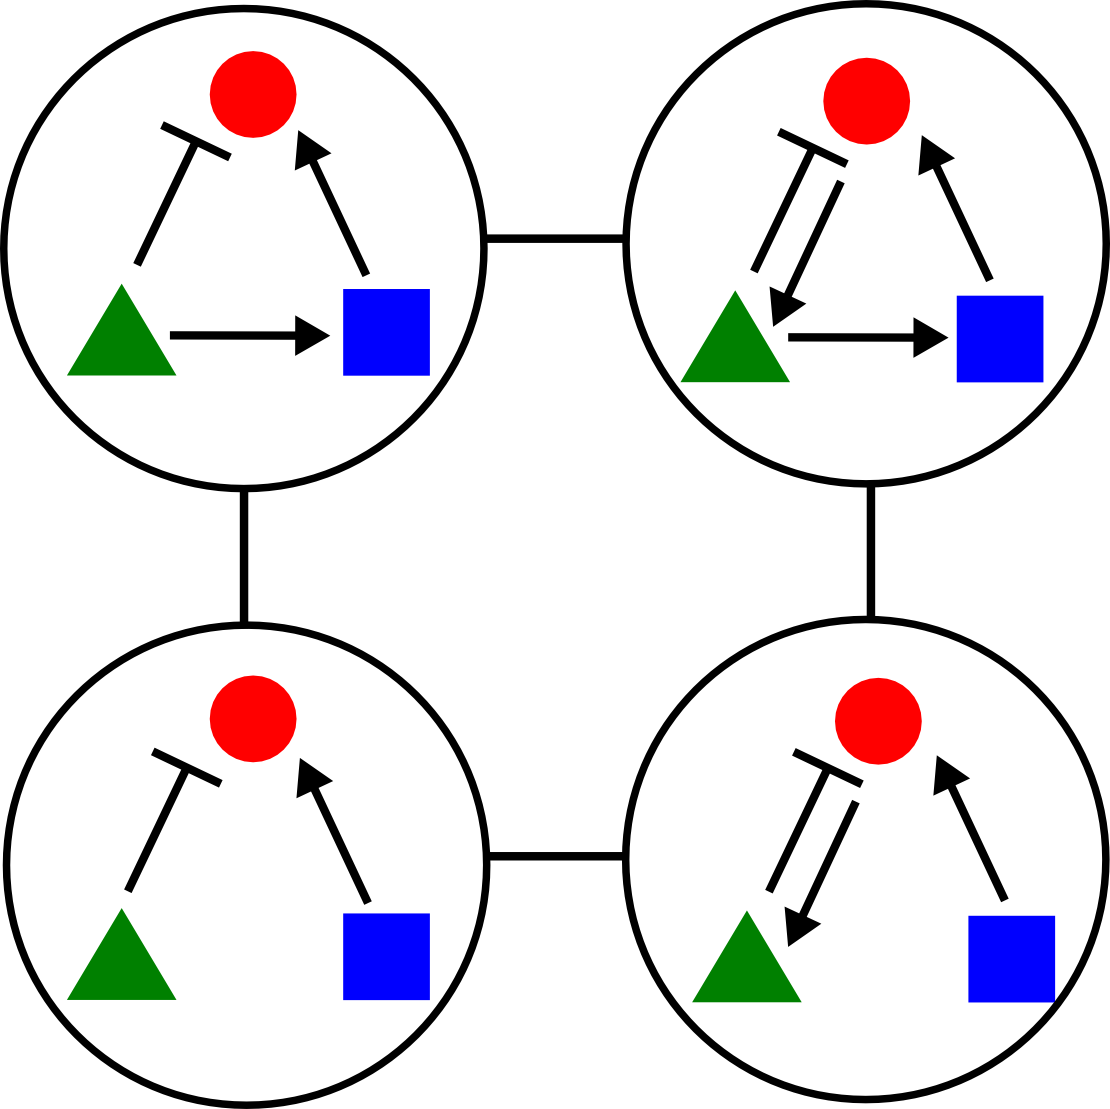
\includegraphics[width=5cm]{./Images/GRNs.png}
%  \centering
%  \caption{
%  Some GRNs . Cotterel and Harpe calculated... \citep{Cotterell2010}
% }
%  \label{fig:GRNs}
%\end{figure}
%%%%%%%%%%%%%%%%%%%%%%%%%%%%%%%%%%%%%%%%%%%%%%%%%%%%%%%%%%%%%%%%%%%%%%%%%%%%%%%%%%%%%%
%
%\subsubsection{Complexity in terms of dynamical systems theory}
%
%Dynamical systems theory (DST) has been proposed as an alternative to analyse complex GRNs. DST is branch of mathematics used to describe complex systems usually with differential or difference equations. 
%In developmental biology, DST has been used to identify the set of networks that can produce a certain output. 
%For example, Cotterel and Sharpe defined all the possible regulatory topologies of a simple three-gene GRN (in which each gene can activate or inhibit the expression of any gene including its own), and then identified the subset of network capable of the formation of a single stripe of gene expression in a one-dimensional cell array. They determined that only 471 of the possible 3379 topologies were capable of such task \citep{Cotterell2010}.
%
%
%Estimating the combinatorial possibilities of a small set of regulatory genes, considering that each gene can regulate (whether positively or negatively) more than one gene's expression in addition to its own, could result in an astronomic number of possible gene topologies (see Figure \ref{fig:GRNs}).
%Also feedback effects and non-linear regulation of gene expression make the prediction of changes in regulatory states hard or even impossible to predict \citep{Jaeger2014devmech}.
%
%To overcome this limitations, some authors have propose to use dynamical systems theory, which deals with a complex system with many interacting components (a dynamical system), by representing its state as a point in a multidimensional space \citep{Alberch1991,ForgacsandStuartA.Newman.2005,Jaeger2014devmech}. 
%To illustrate this we could think of a specific cell type, with \textit{n} number of genes, which its cell state depends on the expression of each of the genes.
%The simpler case we could imagine would be a cell with only two genes. In this case, the cell would be in a two-dimensional "state space" (also called "phase space").
%
%Importantly, the dynamical system is governed by the relations between its components \citep{ForgacsandStuartA.Newman.2005}. In our example the relations would be represented by the interaction between genes, namely the gene regulatory network (GRN). 
%If in our example the expression level of one gene is affected by the expression level of the other gene, the system will not stay in any particular state, but it will change until it reaches a "stable steady state", in which the level of both genes are at equilibrium. 
%Given a specific GRN, the number of stable states would represent the possible differentiation states a cell can achieve (REF Slack book)
%
%Many modifications of the GRN would not have consequences in the ultimate differentiation state, as it will converge to the same "attractor" point.
%However, some modifications (or mutations) could produce a change in the "state space" leading to the formation of a new stable state (i.e., a new cell type).
%So within the framework of the dynamical systems theory, and keeping the number of cell types as our measure of complexity, there would be an increase in complexity when a mutation would change the gene regulatory machinery so that a new stable steady state is formed.


\subsubsection{McShea's view of complexity}

Daniel W. McShea has provided some useful definitions of biological complexity. According to one of his definitions, "complexity of an organism is the amount of differentiation among its parts or, where variation is discontinuous, the number of part types" \citep{McShea1996,McShea2015}.
This definition can be used at different hierarchical levels of biological organization, e.g., tissues, cells, genes.
Indeed, a measure of morphological complexity that has been favoured by some authors 
%(perhaps because of its intuitiveness), 
is the number of cell types that compose an organism \citep{Valentine1994,Bell1997,Bonner2004}.
This definition of complexity is not exempt of complications, as there is no clear criteria of how to define a cell type or how to determine, during development, when a new cell type has formed.

Importantly, with this definition (complexity as the number of parts), the complexity at different levels are not necessarily correlated.
%
%These "parts" might be body segments (e.g., of an insect) or genes.
%It is evident that these definitions are problematic.
%It is doubtful to say that some centipede is more complex than a beetle, just based in the different number of segments they have.
This lack of correspondence at different levels becomes evident when comparing the number of genes with the number of cell types. Before the release of the first eukaryotic genome sequences, it was expected that the number of genes would correlate with an intuitive perception of organismal complexity, ranking complexity as yeast $<$ nematodes $<$ flies $<$ humans \citep{Hahn2002} (this intuitive notion of complexity correlates with the number of cell types in metazoans; \citealp{Valentine1994}). However, this expectation was proved to be wrong and this lack of correlation between "intuitive complexity" and genes number was called the "G-value paradox" \citep{Hahn2002}.
%This is related with the already acknowledged lack of correlation between the number of coding-genes and morphological complexity, 
%This lack of correspondence, 
%sometimes referred as the "G-value paradox"
%	\citep{Hahn2002}.
%Some decades ago, there was the expectation that the morphological complexity should correlate with the number of genes in an organism. 
%With the release of the first eukaryotic genome sequences, such correspondence was not observed.
Before that, the lack of correspondence between genome size and organism complexity (using again an intuitive notion of complexity),  or "C-value paradox", was also noted.
The lack of correspondence between the number of genes with an intuitive notion of complexity is now partly explained by some authors by the amount of post-transcriptional regulation \citep{Sempere2006}.
This paradox can also be partially explained by the currently acknowledged notion that during development, genes do not act individually, but they act within gene networks. Therefore, the phenotypic complexity is affected not only by the number of genes involved in its development, but also by the topology of the gene networks.

This relates to McShea's distinction between "object complexity" that refers to the number of parts of a system and "process complexity" that refers to the interaction among parts in a system \citep{McShea1996}.
%An alternative definition of complexity includes not only the "number of parts" but also the "interaction among parts" 
%	\citep{McShea1996,Arthur2010}.
This could be illustrated with the number genes (object complexity) and the number of gene-gene interactions (process complexity). Gene-gene interactions would refer to the regulation of a gene expression by the binding of another gene product (transcription factor) to its promoter region.
Using this definition, two different organisms would have the same object complexity if they have the same number of genes, but one would have a higher process complexity it has more gene-gene interactions than the other.


%%%%%%%%%%%%%%%%%%%%%%%%%%%%%%%%%%%%%%%%%%%%%%%%%%%%%%%%%%%%%%%%%%%%%%%%%%%%%%%%%%%%%%%%%%%%%%%%%%%%%%%%%%%%%%%%%%%%%
\subsection{Complexity Increase in Development and Evolution}

The increase in complexity in an organism during embryogenesis is probably one of the most intuitive processes of animal development.

It is commonly seen even as one of its defining characteristics.
Eric H. Davidson described the progressive increase in complexity as the "essence" of development \citep{Davidson2001}. Despite of the widely accepted view of complexity increase in development, there is no consensus of how to define it, much less on how to quantify it \citep{susan2000ontogeny}.

%One of the most accepted definitions of complexity is the number of cell types in an organism \citep{Valentine1994,McShea1996,Bell1997,Bonner2004,Arthur2010}.

Using the number of cell types, the increase of complexity during development is self-evident: in vertebrates, the embryo begins with one cell type (the zygote) and concludes with more than 200 cell types \citep{Alberts1994}. 

%Using the number of cell types again as a proxy of morphological complexity, it can be said that during metazoan development, complexity increases as the zygote divides and differentiates into an adult with multiple cell types. 

%This definition of complexity is not exempt of complications, as there is no clear criteria of how to define a cell type or how to determine when a new cell type has formed during development. 
%For example, it could be that at the morphological level a cell seems to be undifferentiated, but when isolating it from its neighbour cells, it differentiates in an autonomous way into a specific cell type, suggesting that the cell fate was already determined without the necessity of further interactions with other cells.
%
%In addition, this definition does not take into account that embryos do not only get more cell types, but they also get organized in specific patterns in space and time in the embryo, which also could be considered as an increase in complexity over developmental time.
%
%The notion of an increase in complexity during embryogenesis is tightly related to the concept of embryo compartmentalization.


%%%%%%%%%%%%%%%%%%%%%%%%%%%%%%%%%%%%%%%%%%%%%%%%%%%%%%%%%%%%%%%%%%%%%%%%%%%%%%%%%%%%%
%\clearpage
%
%\setcounter{figure}{2}% Modify counter of figure so it maches the order, as here im not using \begin{figure}
%
%\begin{mdframed}[style=boxstyle,frametitle={Box1. On the relationship between the increase of complexity in Evolution and Development}]\label{Box1:Evo_complexity}
\subsubsection{ On the relationship between the increase of complexity in Evolution and Development}
The connection between the increase in complexity during development and evolutionary time has been largely discussed.
Haeckel was one of the first who made explicit hypotheses about the connection between the development and evolutionary patterns in his "Biogenetic Law" (see Box 1).
%
These laws imply that the increase in complexity we see during development is a reflection of a similar increase in complexity that has occurred through evolution.
%
Early views of evolution saw the increase in complexity as inexorable, with all the species descending from simpler ancestral forms \citep{lamarck1809zoo,haeckel1874menschen}, and with the human species as the latest and more perfect product of the evolution of animals \citep{haeckel1874menschen}.


Recent views recognize that complexity can increase or decrease in a lineage.
Using the number of cell-types as complexity measure, there are clear examples of taxa that have decreased their complexity over time, specially in parasites \citep{Canning2003,Arthur2010} (although morphological simplification can not be considered universal in parasitic taxa \citealp{poulin2011evolutionary}). On the other hand, there are many lineages that have remained unicellular (i.e., their complexity would have remained constant), while some lineages (e.g., vertebrates) have increased their complexity. Hence, it seems that there is no unique trend to increase the complexity over time, in other words, the complexity of a specific lineage might decrease, increase or stay the same (see Figure \ref{complexity_trend}).
%%%%%%%%%%%%%%%%%%%%%%%%%%%%%%%%%%%%%%%%
\par
{\centering
  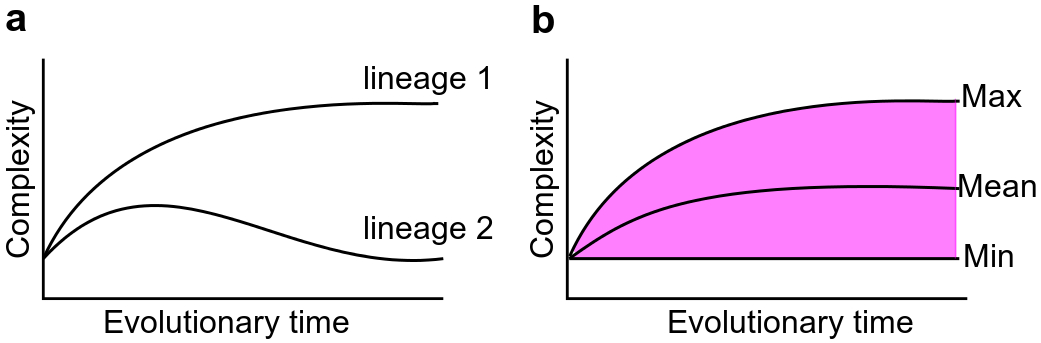
\includegraphics[width=0.8\textwidth]{./Images/complexity_min.jpeg}
  \centering
  \captionof{figure}{Two lineages with different complexity change through their evolutionary trajectories.
  b) Representation of the minimum, mean and maximum complexity of many lineages over evolutionary time in which the minimum stay constant while the mean and maximum increase.
Redrawn from \citep{Arthur2010}.}
\label{complexity_trend}
}
\par
%%%%%%%%%%%%%%%%%%%%%%%%%%%

If we consider uni-cellularity as the minimum complexity, it can be said that minimum complexity has remained more or less constant in evolution, as unicellular organisms like bacteria, have been present since 3.5 billion years. However, if we consider instead maximum complexity a trend for increasing such complexity would be apparent, as complexity would have increased with the appearance of simple multicellular organisms (only few cell types) and would have further increased until the appearance of organisms composed of hundreds of cell types. For some authors this apparent trend of increasing complexity is the product of natural selection \citep{bonner1988evolution,Carroll2001}.
%This notion can lead to circular reasoning, saying that organisms are complex because they have been selected for that, and that they have been selected because they are complex. \textbf{EXPLICAR MEJOR}

In contrast, other authors consider that this apparent trend does not necessarily imply that it has been selected for \citep{McShea2015}, and that this trend might appear even in scenarios without natural selection. 
For example, if we consider an evolutionary scenario in which the complexity of the organisms follow a random walk scenario without any selection regime but with the condition of a lower boundary (i.e., is not possible to have less than once cell), and starting from unicellular organisms, we will see an increase of the maximum complexity, with an initial increase in the mean complexity (in a random walk the expected distance of a point after $n$ time steps is $\sqrt[2]{n}$, but when considering many points the mean distance at any time point is 0) \citep{gould1996fullhouse}.
%, the mean and maximum would show a trend towards increasing complexity \ref{boxfigure} given that there is a minimum complexity requirement (it is not possible to have less than one cell) \citep{gould1996fullhouse}.
%\textbf{DESCRIBIRLO MAS CLARAMENTE}
%\end{mdframed}
%%%%%%%%%%%%%%%%%%%%%%%%%%%%%%%%%%%%%%%%%%%%%%%%%%%%%%%%%%%%%%%%%%%%%%%%%%%%%%%%%%%%%

\subsubsection{Compartmentalization in development}

The notion of an increase in complexity during embryogenesis is tightly related to the subdivision of the embryo in different parts during development. 
In here, I will refer to this process as the compartmentalization of the embryo. 
The different parts of the embryo could be defined based on the cell-phenotype or gene expression profile.

It is usually considered that the earliest subdivisions that are formed in the embryo define the main body axis, i.e., the anterior/posterior (A/P) and dorsal/ventral (D/V) axes.
	\nomenclature{A/P}{anterior/posterior}
	\nomenclature{D/V}{dorsal/ventral}
Later on, smaller subdivisions of the embryo would be formed, e.g, limbs, eyes or internal organs. In this manner as development proceeds, it is expected that spatial subdivisions would be progressively specified at an increasing finer resolution \citep{Davidson2001}.
%However, the definition of pattern is different from the compartments one, in that the a pattern transformation does not necessarily involves changes in gene expression. A new pattern could be formed by a morphogenetic process, e.g., migration.
%\hfill \break
%This progressively compartmentalization is expected to be reflected at the level of gene expression: genes would be expressed ubiquitously at very early development, then some would be expressed in large regions in the embryo defining the main embryo axes and in later developmental stages some genes would be expressed in cell-specific or tissue-specific manner.
Furthermore, the increasing compartmentalization of the embryo during development can be conceptualized as the progressive spatial restriction of gene expression to subsequently smaller regions in the embryo.
Sean Carroll defines this process\citep{Carroll2001} as:
%%%%%%%%%%%%%%%%%%%%%%%%%%%%%%%%%%%%%%%%%%%%%%%%%%%%%%%%%%%%%%%%%%%%%%%%%%%%%%%%%%%%
\begin{enumerate}
\item In early development, genes have a broad expression in the embryo and define the main axes of the body.
\item Later, genes define smaller compartments like organs and appendages (field-specific selector genes).
\item Finally, genes become expressed in specific cell types like muscle and neural cells (cell-type specific selector genes). 
\end{enumerate}
%%%%%%%%%%%%%%%%%%%%%%%%%%%%%%%%%%%%%%%%%%%%%%%%%%%%%%%%%%%%%%%%%%%%%%%%%%%%%%%%%%%%
It is important to note that this would imply that, in general, the area of expression of a gene in the embryo would decrease during development (relative to the area of the whole embryo).

It is important to mention that compartmentalization (as the embryo subdivision) used in here is different from the most commonly and widely accepted definition of developmental compartment proposed by \citet{Garcia-Bellido1973}.
They defined compartments as differentiated populations of cells (at the gene expression level) that do not intermix between them and that these are formed from initially homogeneous contiguous cells. 
The definition used in here is related to the one of Garcia Bell\'{i}do et al., but in contrast to it, does not rely on the identification of a boundary formation between different cell populations that would prevent cell mixing between them.
%\citet{Garcia-Bellido1973} proposed this concept after an experiment using clonal analysis, in which they found that different parts of the fly wing were subsequently determined in the imaginal disc by the formation of differentiated populations of cells that do not intermix between them.
%They demonstrated that the imaginal disc is initially divided in two compartments: anterior and posterior that subdivide into smaller compartments that pre-define specific parts of the adult wing.  It was later proposed that the compartmentalisation was specified by a genetic code like a ZIP address \citep{Garcia-Bellido1979}.

%\subsubsection{Developmental pattern}
%A developmental pattern can be defined as the specific distribution of cell types in a specific temporal window of embryonic development \citep{Salazar-Ciudad2004}. 
%Therefore, development can be conceptualized as the continuous transformation of one pattern into another.
%This relates to the compartments definition, as the earliest pattern transformations usually establish the main axis or "compartments" of the embryo. For example, the anterior/posterior (A/P) and dorsal/ventral (D/V) axes in the fruit fly.
%	\nomenclature{A/P}{anterior/posterior}
%	\nomenclature{D/V}{dorsal/ventral}
%Later pattern transformations would define smaller compartments of the embryo, e.g, limbs, fingers  or internal organs.
%However, the definition of pattern is different from the compartments one, in that the a pattern transformation does not necessarily involves changes in gene expression. A new pattern could be formed by a morphogenetic process, e.g., migration.
%\hfill \break
%As development proceeds, spatial compartments are progressively specified at an increasing finer resolution \citep{Davidson2001}.
%Thus, a great proportion of pattern transformation involve the partition of specific embryo compartments into smaller sub-compartments.
%
%The compartmentalization of the embryo can be considered then an intrinsic property of development and could be used as a proxy of complexity.


\subsubsection{Complexity at the molecular level}

For some authors, the increase in complexity in an organism during development (reflected by the increase of number of cell types), should be associated with an underlying complexity at the molecular level \citep{Davidson2001,Arthur2010}, following the reasoning that:
%If we consider again the number of cells as the complexity measure, it could be expected that the increase in complexity over developmental time should be associated with an underlying increase in complexity at the molecular level \citep{Arthur2010}, following the reasoning that:

%%%%%%%%%%%%%%%%%%%%%%%%%%%%%%%%%%%%%%%%%%%%%%%%%%%%%%%%%%%%%%%%%%%%%%%%%%%%%%%%%%%%
\begin{enumerate}
\item In development, complexity increases with time as new cell types form.
\item Different cell-types are characterized by the differential expression of genes.
%\item Therefore, the more cell-types an organism is formed of, the more different combinations of expressed genes there has to have (with the gene regulatory complexity this must entail).
\item Therefore, a complex organism (composed of many cell-types) has to contain a complex gene expression regulatory machinery to produce the different combinations of expressed genes in each cell-type \citep{Davidson2001}.
\end{enumerate}
%%%%%%%%%%%%%%%%%%%%%%%%%%%%%%%%%%%%%%%%%%%%%%%%%%%%%%%%%%%%%%%%%%%%%%%%%%%%%%%%%%%%
%
%The above reasoning has lead to some researchers to propose that the complexity of an organism resides in the regulatory machinery that ends into the differentiation of the diverse cell types \citep{Davidson2001}. 

%Furthermore, the increasing compartmentalization of the embryo during development can be conceptualized as the progressive spatial restriction of gene expression to subsequently smaller regions in the embryo.
%Sean Carroll defines this process\citep{Carroll2001} as:
%%%%%%%%%%%%%%%%%%%%%%%%%%%%%%%%%%%%%%%%%%%%%%%%%%%%%%%%%%%%%%%%%%%%%%%%%%%%%%%%%%%%%
%\begin{enumerate}
%\item In early development, genes have a broad expression in the embryo and define the main axes of the body.
%\item Later, genes define smaller compartments like organs and appendages (field-specific selector genes).
%\item Finally, genes become expressed in specific cell types like muscle and neural cells (cell-type specific selector genes). 
%\end{enumerate}
%%%%%%%%%%%%%%%%%%%%%%%%%%%%%%%%%%%%%%%%%%%%%%%%%%%%%%%%%%%%%%%%%%%%%%%%%%%%%%%%%%%%%
%
%It is important to note that this would imply that, in general, the area of expression of a gene in the embryo would decrease during development (relative to the area of the whole embryo).

%%%_-----------------------------------
%
%At the molecular level, the definition of "interaction among parts" and "number of parts" can be easily associated, as the the differential gene expression in the various number of cell types are determined in great manner by the interaction of between gene products and their \textit{cis}-regulatory regions (DNA regions usually close to a gene which contains specific sequence motifs where proteins bind and affect its expression).
%%
%The interaction between genes and their \textit{cis}-regulatory regions is also referred as gene regulatory networks (GRNs) or "regulatory architecture" of the genome \citep{Davidson2001}.
%	\nomenclature{GRN}{Gene Regulatory Network}%\textit{cis}-regulatory regions 


%\textbf{Other} authors highlight the importance of modules in facilitating the evolution of complex forms \citep{Carroll2001a}.


\paragraph{Gene expression regulation}

It is widely acknowledged that the spatio-temporal regulation of gene expression in development is crucial for the progressive compartmentalization of the embryo. 
%After acknowledging the importance of the spatio-temporal regulation of gene expression in development, 
%Therefore, it is useful to identify which type of genes are directly involved in this process. 
More than fifty years ago, Jacques Monod and Fran\c cois Jacob \citep{Jacob1961} published in a seminal work a model of the genetic regulatory mechanism in bacteria.
The most important conclusion of this paper was the existence of "regulator" genes that control the production rate of proteins from "structural" genes, and that mutations in "regulator" genes affect the regulatory mechanism but not the structure of the regulated protein. In the same paper they suggested that these regulator genes may affect the synthesis of several different proteins \citep{Jacob1961}.

Nowadays the process of gene activation is known in great detail. The  "regulator genes" Jacob and Monod studied are transcription factors, proteins that bind to DNA to promote or repress the transcription of a gene.

This transcriptional regulation represents however only one level of gene expression regulation. There are many other mechanisms that regulate the production of gene products. These include 3' untranslated regions (UTR) \citep{Grzybowska2001}, small interference RNAs (siRNAs) \citep{Filipowicz2005}, translational \citep{Kozak1992,Kapp2004} and post-translational \citep{Mann2003} regulation of gene expression.
	\nomenclature{miRNAs}{Micro RNAs}
	\nomenclature{siRNAs}{Small interference RNAs}

At least two regulatory levels have been explicitly suggested to have a causal role in the increase in complexity in different lineages:  transcriptional regulatory level (as mentioned above) \citep{Davidson2001} and miRNAs. The role of miRNAs (non-coding RNA molecules that negatively regulate gene expression) was proposed after the observation that miRNAs are found only in protostomes and deuterostomes and not in sponges or cnidarians, and that they are specifically expressed in certain cell-types, tissues or organs \citep{Sempere2006}.
%
It could be expected however that the complexity of an organism could be reflected at any level of gene expression regulation, whether transcriptional, post-transcriptional, translational or post-translational.

%Additionally to all these regulatory levels that occur within a cell, the spatio-temporal regulation of gene expression depends on signalling between neighbouring cells and morphogenetic events \citep{Gilbert2014}. Importantly, cell-cell signalling can affect the transcriptional state of a cell (through a signalling pathway). Additionally, the specific response of a signalling event is dependent on the transcriptional state of the cell.

%The molecule network involved in cell-cell communication, from the reception of a extracellular signal to the ultimate transcription of genes (usually going through many intermediate signal "transducers"), is known as a signalling pathway.


%
%%%%%%%%%%%%%%%%%%%%%%%%%%%%%%%%%%%%%%%%%%%%%%%%%%%%%%%%%%%%%%%%%%%%%%%%%%%%%%%%%%%%%%
%\begin{figure}[h]
%  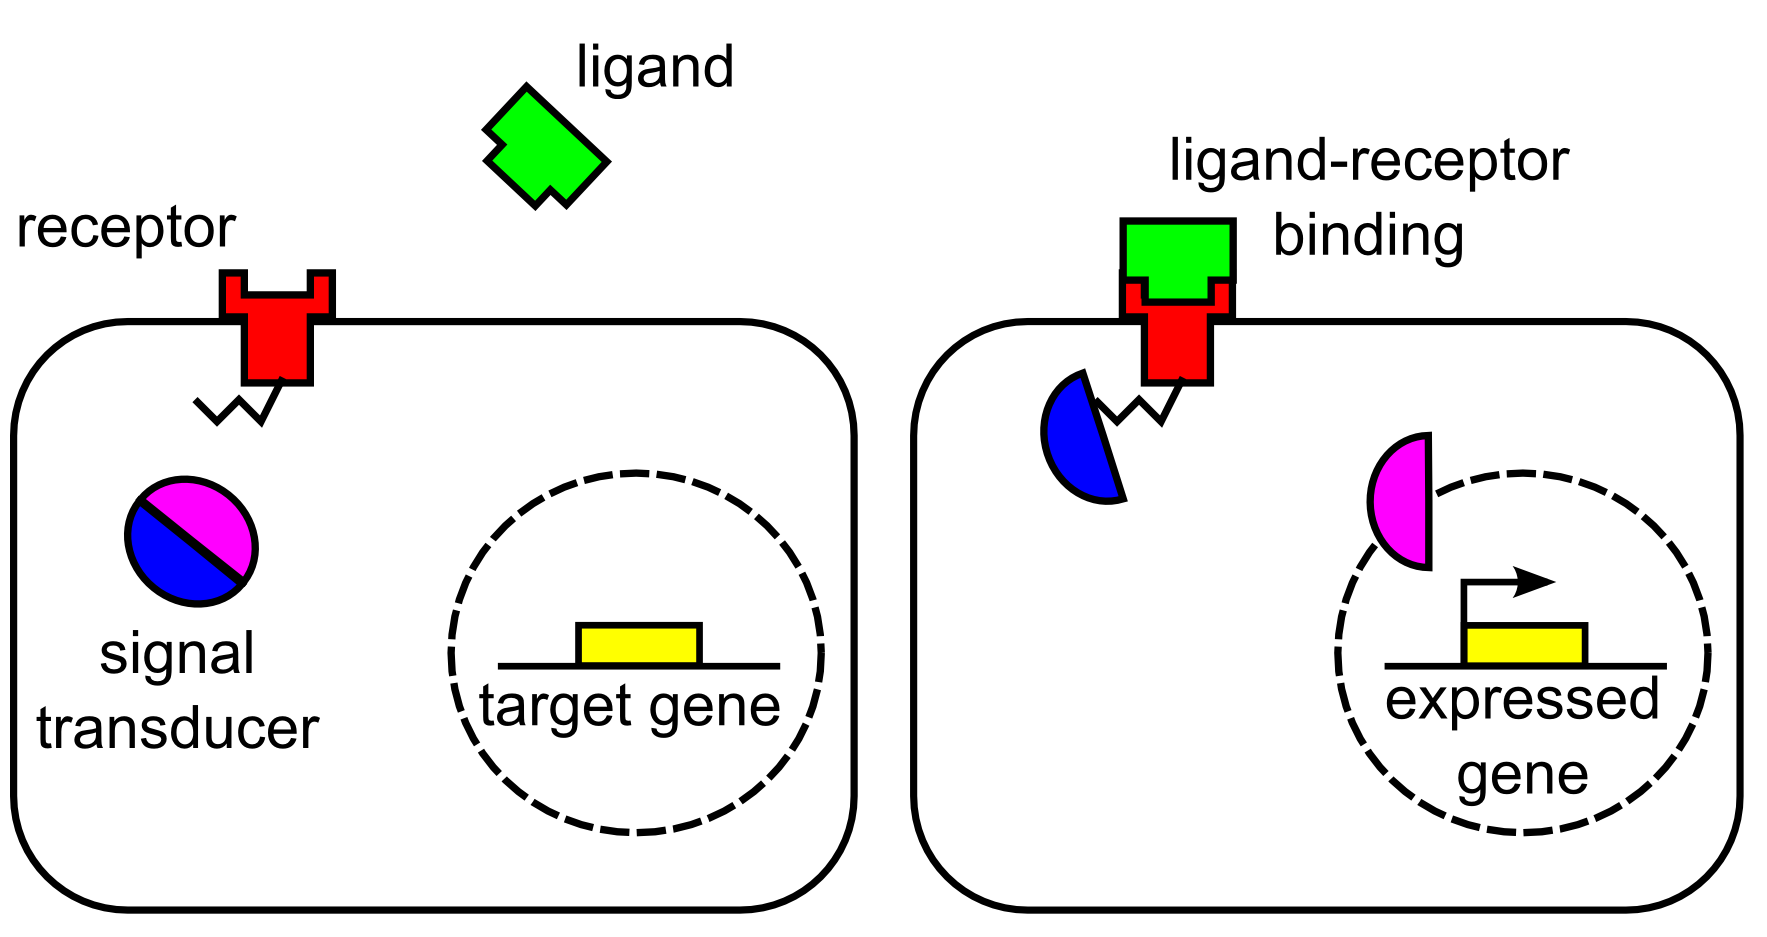
\includegraphics[width=10cm]{./Images/signalling.png}
%  \centering
%  \caption{
%  Scheme of an hypothetical signalling pathway. Left: The extracellular ligand (green) is not bound to the membrane receptor (red) so the signal transducer protein (blue/magenta) is inactivated. In the nucleus (dashed circle) the target gene (yellow box) is inactive. Right: As the ligand binds to the receptor, the cytoplasmic domain (depicted as a zigzag tail) of the receptor change to an active conformation, cleaving the signal transducer. Part of the signal transducer acts as a transcription factor, going into the nucleus where activates the transcription of the target gene after binding to its regulatory region.
% }
%  \label{fig:Signalling}
%\end{figure}
%%%%%%%%%%%%%%%%%%%%%%%%%%%%%%%%%%%%%%%%%%%%%%%%%%%%%%%%%%%%%%%%%%%%%%%%%%%%%%%%%%%%%%
%
%\paragraph{Transcription factors} The transcription factors (TFs) are proteins that bind to specific regulatory regions, to induce or repress the expression of a gene.
%Based on the secondary structure of the protein binding domain, TFs can b e classified in four main families: helix-turn-helix, helix-loop-helix, zinc finger and leucine zipper (\citep{Carroll2001}.
%	\nomenclature{TF}{Transcription Factor}
%	
%The members of each family has been recognised in playing different roles in development. For example, it has been observed that in diverse metazoan species C2H2 zinc-figers TFs are over-represented in early development, as opposite to Homeobox TFs which are under-represented in the same period \citep{Schep2013}.
%Hox genes (a subset of the Homeobox TF family) are involved in the A/P patterning of many metazoan groups. Intriguingly, these genes were found to have spatial collinearity in mice and flies (REF). That means that the A/P expression of the Hox genes reflects their physical order along the chromosome.
%At the time of its discovery, collinearity of Hox genes were considered as a master plan for A/P patterning in animals (REF).
%However, after Hox genes were investigated in more species it became clear that in some species with Hox genes collinearity is not always present, and some species do not have Hox genes at all (REF).
%
%\paragraph{Signalling pathway genes} Signalling pathways are usually a complex network of molecules including extracellular diffusible signals, membrane receptors, intermediate signal transducer molecules and transcription factors.
%Signalling pathways usually begin with a extracellular signal that causes a conformational change in its cell membrane receptor after binding to it.
%The new conformation results in enzymatic activity in the cytoplasmic domains of the receptor protein, that phosphorylate other cytoplasmic proteins.
%Finally, one or more activated transcription factors induce or repress specific gene activity \citep{Gilbert2014}.
%
%Signalling pathways recurrently used during animal development are the Wnt, FGF and Shh pathways (for a detailed description of each signalling pathway, see \citep{Gilbert2014}.
%For example, the Shh pathway plays a fundamental role in the fruit fly segment polarization(REF) and wing development (REF), and in vertebrate limb (REF) and tooth development \citep{Jernvall2000b}.

\subsection{Shape complexity}

Until this point, I have focused on the concept of compartmentalization 
%(and the molecular regulatory mechanisms that might be responsible for it) 
as one aspect that reflects the increase in complexity during development.
Another aspect that is intuitively related to the increasing embryonic complexity is the shape (or form) of the embryo. 
Focusing on the shape of the embryo, embryonic development can be thought as a process that starts with a simple spherical or oblate fertilized egg and that ends with complex shapes and forms (in the adult or larva) \citep{Forgacs_Newman2005}. 

In addition to the external shape of the embryo, the shape complexity of its internal structures (e.g., organs) is expected to increase during development \citep{Sharpe2003}. %Also, it could be expected that when analysing a large number of genes, the shape complexity would increase at a statistical level.

However, it is not always possible to appreciate the morphological change of inner structures at simple view. The first attempts to describe the shape of internal organs during the development in vertebrates was in the 19th century, and it required  section cutting and wax reconstruction \citep{Hopwood2007}. The use of staining techniques have facilitated the visualization of the inner morphology of the embryo. Techniques such as the horseradish peroxidase staining facilitated not only the visualization of the inner morphology, they were also crucial to create the first fate maps, while being able to trace the cell-lineage of different organs. 

Since now is known that many genes are expressed in a tissue/cell type specific manner, another useful technique to visualize inner structures is the use of labelling techniques that highlight the distribution of such tissue-specific gene products (e.g., whole-mount in situ mRNA hybridization or immuno-histochemistry techniques). 
If the embryo external and internal morphology are expected to increase their spatial complexity, and some gene expression patterns (visualized with a labelling technique) is expected to correspond to specific regions (e.g., internal organs) or the whole embryo (in case the expression is ubiquitous), consequently, the shape of gene expression patterns could be used to describe the morphological complexity of the embryo. It is important to mention that even when some gene expression patterns might reflect (and could partially explain) the organ distribution and form, usually there is no simple one-to-one correspondence between genes and organs. Indeed, many developmental genes are expressed in many organs at different developmental stages.
% When analysing the shape of a gene expression through development, it could be that the expression pattern: 1) does not change its complexity, 2) becomes more complex, or 3) becomes less complex.
%also be expected to increase its spatial complexity during development. 

The study of morphometrics refers to the quantitative analysis of morphological shape. In the last decades, morphometric tools have been used widely as a tool to quantify, characterize and compare biological shapes \citep{JamesRohlf1993}. In the next paragraphs I will briefly explain the most important morphometric methods. For an extensive review, see \citep{Bookstein1997,Dryden1998,Zelditch2008,Slice2005}.


\subsubsection{Morphometrics}

In morphometrics, shape refers to the geometric properties of an object that are invariant to location, scale and orientation \citep{Slice2005}. Many of the modern morphometric analyses are based on the use of "landmarks", which refer to precisely located points that establish a clear one-to-one correspondence between the samples under study \citep{Klingenberg2010}. To extract only the shape information from the landmarks, the variation in size, position and orientation are usually removed with a technique called "Procrustes superimposition" \citep{Dryden1998}.
Although there are many different morphometric methods, they can be divided in four main categories: "traditional morphometrics", "geometric morphometrics", outline analysis and surface analysis \citep{Slice2005}.

The \textbf{"traditional methods"} refer to the application of multivariate statistics, like Principal Component Analyses (PCA), to the direct measurement of lengths, widths or ratios of specific structures. Some typical applications of these methods are the classification of species or sexes \citep{Jolicoeur1960} using lengths, widths or angles between landmarks \citep{Dryden1998}.
	\nomenclature{PCA}{Principal Component Analysis}

\textbf{Geometric morphometrics} analyses use instead geometric coordinates of morphological landmarks  \citep{Mitteroecker2009,zelditch2012geometric}. As with the traditional methods, PCA can be used for analysing the shape variation in the dataset \citep{Klingenberg2010}.
A variant of landmark analyses is the use of "semi-landmarks". Semi-landmarks are equally spaced points around an outline, usually between "real landmarks". Semi-landmarks are therefore used when only a few landmarks are recognisable. For example, in the analysis of the shape of hands, "real landmarks" can be placed in the tip of the fingers, and the semi-landmarks would be placed along the hand outline. After recording the semi-landmarks, procrustes superimposition and multivariate analyses can be used as with ordinary landmarks \citep{Dryden1998}.

\textbf{Outline analyses} are specially relevant when it is not possible to identify comparable landmarks between samples. 
%
One type of outline analyses is the Elliptic Fourier description \citep{Kuhl1982}, which uses an orthogonal decomposition of a curve into a sum of harmonically related ellipses \citep{Ferson1985}. The extracted harmonics can then be analysed with PCA. A classical example of the Fourier description is the analysis of mussel shells (which can be represented as a closed outline) done by \citet{Ferson1985}.
% 
Another outline method is the Eigenshape analysis, which uses outline coordinates to calculate angles between points to provide a map around the outline. More specifically, shape is represented as the shape function $\phi^{*}(l)$, the normalized net angular change in direction $\phi$ at each step around the perimeter $(l)$ (the normalization can be based on the deviation from a circle, or from the sample mean) \citep{Lohmann1983}. Then, the major directions of observed and measured shape variation is analysed by means of
eigenanalysis. 
Eigenshape analysis (a type of Principal Component Analysis) derives a set of empirical orthogonal shape functions by an eigenfunction or PCA of a matrix of correlation between shapes \citep{Lohmann1983}.


\textbf{Surface analyses} are used when comparing 3D objects (usually represented as Cartesian coordinates $x$,$y$ and $z$ of points on the object's surface) with limited landmark information. For example, a vertebrate skull has many identifiable anatomical landmarks in the face but only a few can be defined unambiguously on the smooth braincase \citep{Mitteroecker2009}. In order to deal with this, \citealp{Gunz2005} extended the use of 2D outline semi-landmarks to 3D surfaces. 3D semi-landmark methods are based on allowing the points to "slide" along the surface until some measure of shape difference (e.g., bending energy of a thin-plate spline) among the configurations is minimized \citep{Mitteroecker2009}.


\subsubsection{Topographic anaytical methods}
\label{DNE_explanation}

Another approach to 3D surfaces is the use of topographic analytical methods. These methods, which apply concepts from Geographic Information Systems (GIS), have been used to quantify teeth surfaces as if they were landscapes \citep{jernvall1999laser,Winchester2014}.  
	\nomenclature{GIS}{Geographic Information Systems}

New topographic analytical methods that do not rely on GIS have been recently developed. This is the case of the Dirichlet normal energy (DNE), a method for quantifying surface bending using concepts from differential geometry \citep{Bunn2011}. This method quantifies the deviation of a surface mesh from being planar \citep{Bunn2011}. A brief explanation of the DNE follows, for a complete description see \citep{Bunn2011,Winchester2016}. For each polygon in the surface mesh, DNE calculates its energy value $e(p)$. The energy value quantifies change in the normal map around a polygonal face. The DNE value of the whole surface is the sum of all the energy values $e(p)$ of the polygonal mesh surface. DNE values increase with both convexities and concavities on a surface. This measure has been used in the shape quantification of mammals tooth crowns, for dietary inference \citep{Bunn2011}.

%The energy value e(p) quantifies change in the normal map around a polygonal face. The calculation of the energy value e(p) of a polygon can be exemplified with a schematic diagram as in Fig. 2B. First, the polygon is characterized by vectors u and v, which represent the edges of the polygon. Then, normal unit vectors are estimated as the normalized average of normal vectors of the triangle faces adjacent to each vertex (Fig. 2B). If vertex normals are translated to a common origin point, their end points form a polygon with edge vectors nu and nv, which represents the spreading of nu and nv (Fig. 2C). In a simplistic way, DNE can be defined as the spreading of nu and nv relative to the spreading of u and v. Polygons on more curved surfaces will produce greater relative spreading of nu and nv (Bunn et al., 2011; Winchester, 2016). 
%
%
%\subsection{On the complexity measures used in this work}
%
%\textbf{ESTAS MEDIDAS SON TRES MEDIDAS DE COMPLEJIDAD. LA DE ROUGHNESS ESPECIALMENTE.
%}
%
%\subsubsection{Compartmentalization}
%
%As mentioned before, the process of embryo compartmentalization, or the subdivision of the embryo in different parts during development, is considered to be largely reflected in the expression of the genes in progressively smaller areas. Therefore, a good measure of compartmentalization would be to measure the relative area of expression of all genes during development. Gene expression patterns are usually visualized as a 2D image, which reflects the distribution (seen after an experiment such as mRNA in situ hybridization) of a gene product from a specific anatomical view (e.g., lateral, dorsal).  More recently, methods like 3D imaging technique Optical Projection Tomography  \citep{Sharpe2003,Summerhurst2008} allow to record gene expression patterns in 3D. 
%
%In the case of 2D images, the measure of compartmentalization I use in here is the relative area of the expression of a gene divided by the area of the whole embryo. Therefore, I called this measure "relative area" which ranges from 0 (no expression) to 1 (ubiquitous expression). In the case of a gene expression in 3D, the compartmentalization measure becomes the relative volume of expression.
%Of course it could be said that the compartmentalization of an embryo should not only be reflected in the decrease of the relative area of expression of the genes during development, but also should be reflected in a greater proportion of genes expressed differentially in different parts of the embryo. To account for this, I used a "disparity" measure (explained below), that would be informative in the mean degree of dissimilarity between the different parts of the embryo.
%
%\subsubsection{Disparity}
%
%The disparity measure is related to  McShea's "number of part types" complexity measure. Ideally, the number of cell types, if these could be precisely known, would be a good measure of complexity during development. However, as mentioned before, there is no clear criteria to determine when (at the genetic level) a new cell type is formed during development. 
%Usually, genetic markers are used to determine if a cell (or its descendants) can be considered a specific cell type. This could be the case of anterior or posterior compartment cells within \textit{D. melanogaster} para-segments. For example, the use of wingless (\textit{wg}) or sonic hedgehog (\textit{hh}) in situ hybridization can be used to define if a cell is part of the anterior or posterior compartment. It could be said, however, that the earliest presence of expression of these genes marks the \textit{fate} of the cell, more than the actual cell type. In fact, before the anterior and posterior segment compartments are completely defined, the expression level of these genes changes over time and form a positive feedback to stabilize each other expression. Therefore, a cell that early expresses \textit{wg} would not necessarily differentiate into a posterior compartment if its neighbour para-segment does not express \textit{hh} \citep{Bejsovec1991}.
% 
%Instead of trying to determine the number of cell types during development, an alternative approach would be to quantify how different at the gene expression level are the cells in the embryo. In case it is no possible to have expression for each individual cell, the embryo can be divided in broader regions. To do this, I decided to use a pearson's correlation similarity measure. With this method, the expression of all the genes available in two cells can be compared, giving a value of 1 if all genes have exactly the same expression (their expression is completely correlated), to -1 if all the genes show opposite gene expression (their expression is anti-correlated). An advantage of this method is the possibility to include the information of all available genes, diminishing a possible bias in the gene selection. A further application of this method is the use of clustering algorithms (e.g., hierarchical clustering) to find the main temporal patterns of gene expression in microarray analysis \citep{Eisen1998,Wen1998}. Also, this method can be used to separate cell types based on the genetic differences between them \citep{gohlmann2009gene}.
%
%The pearson's correlation matrix is a measure of gene expression similarity between genes. In here, I was interested on quantifying the difference (i.e., disparity) in gene expression between cells, not on their similarity. Therefore, the disparity between two cells becomes: disparity = 1 - pearson's similarity. The disparity measure ranges from 0 to 2, with a 0 value when the gene expression between cells is exactly the same.
%
%
%\subsubsection{Roughness}
%
%The roughness measure analyses the complexity of the shape of a gene expression pattern. In the case of 2D images, the shape of the gene expression pattern can be extracted as a closed outline formed by the boundaries of gene expression, while in the case of 3D representations, the shape of the expression pattern can be represented as the 3D external surface of the union of the cells that are expressing such gene.
%
%Therefore, a gene expression pattern reflects necessarily the spatial distribution of the cells expressing such gene. When analysing and comparing the shape of many different gene expression patterns (i.e., the cells/tissues with expression are different between genes), there is an obvious impossibility to determine landmark points (whether around a 2D outline or 3D surface) that would establish a clear one-to-one correspondence between them. \textbf{PORQUE?}
%Therefore, a landmark-free method (like outline methods for 2D or surface methods for 3D data) would be ideal to deal with this type of data.
%
%There are practically no studies in the literature that have quantified and compared the shape of gene expression patterns in a systematic manner (one exception is the recent study of \citealp{Martinez-Abadias2016}). In here I will consider that a gene expression pattern is complex if based on the curvature of its 2D contour or 3D surface.
%For 2D gene expression patterns, I used a "roughness measure", that is similar to the shape function $\phi^{*}(l)$ used in eigenshape analyses \citep{Lohmann1983}, as it measures how much the curvature of a closed outline deviates from the angles of a circle of the same perimeter (see methods and study I). 
%In order to use a similar measure of curvature in 3D, I used the Dirichlet normal energy (DNE) described above which quantifies the deviation of a surface from being planar (see methods and study II).
%Importantly, both measures are normalized to remove size and orientation effects.
%
%I selected the roughness measure instead of some other measure outline based method like Fourier analysis because the roughness value gives an intuitive descriptor of complexity, i.e., a value of 1 would be a simple "circle-like" shape, and a value greater than 1 would mean a higher curvature of the outline. \citet{McLellan1998} compared various measures of spatial complexity applied to the outlines of the leaves of many tree species. They included a "margin roughness" measure that is very similar to the one I use here (the difference is that they does not normalize the mean angle by the mean angle of the circle nor he uses different lengths of vectors) and found that there was no marked differences between the margin roughness and a Fourier analysis with up to 64 harmonics (both performed equally well).
%On the contrary, one advantage of the Fourier analysis would be that it is an information preserving algorithm \citep{Pavlidis1980} i.e., it is possible to reconstruct the shape after the analysis, a feature that was not considered relevant for this study. Other feature of the roughness measure is that allows to measure the complexity of shape at different spatial scales (something similar can be done by varying the number of harmonics used in Fourier analysis; \citealp{McLellan1998}). Therefore, it can be tested not only if the complexity of the gene expression shape increases during development, also if this increase is the same at different spatial scales.
%It is important to mention that the aim of this analysis is not to discern which mechanisms (e.g., cell-cell signalling or morphogenetic movements) are responsible for the changes in complexity of the shape of gene expression pattern, but to quantify how this happens during embryonic development.
%
%\subsubsection{The relationship between these measures}
%
%In this work I use three different measures of complexity: relative area/volume, disparity and roughness (analysed with DNE for 3D expression patterns), which are informative of different and independent aspects of complexity. For example, a decrease in the area/volume of gene expression should not be necessarily correlated with an increase in disparity, as the genes that are reducing their expression area could be restricted to the same part of the developing embryo. Only in the case of an embryo with all genes showing ubiquitous expression, there is a clear relationship between disparity and relative area/volume, as the relative area of expression and disparity would be 0 and 1 respectively. If there are however, many genes expressed in only a part of the embryo, these measures are not necessarily correlated. 
%
%%%%%%%%%%%%%%%%%%%%%%%%%%%%%%%%%%%%%%%%%%%%%%%%%%%%%%%%%%%%%%%%%%%%%%%%%%%%%%%%%%%%%%%
%\begin{figure}[h]
%  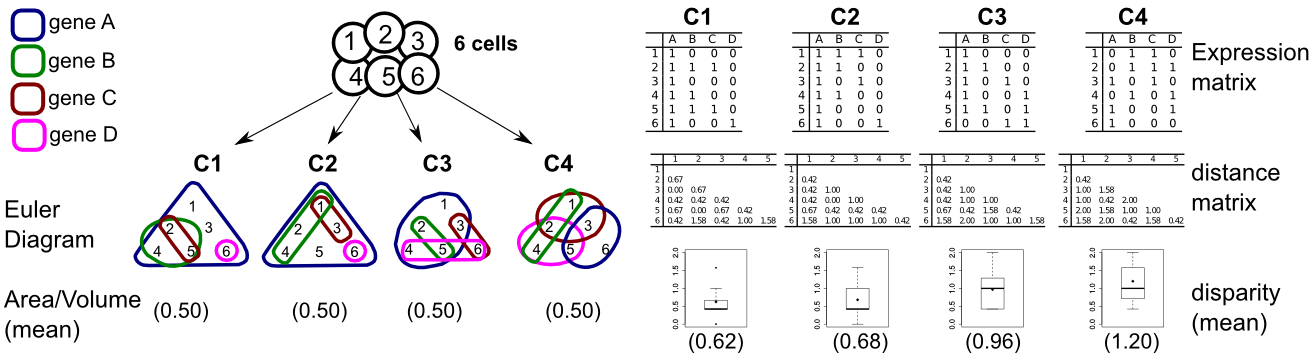
\includegraphics[width=0.95\textwidth]{./Images/measures_relations.png}
%  \centering
%  \caption{\textbf{Relation between area/volume of expression and disparity measures.} An embryo of six cells (top left) is shown expressing four different gene expression combinations (C1, C2, C3 and C4) of four genes (A, B, C and D). All combinations have a mean relative area/volume of 0.5. Each gene expression configuration is represented as an Euler diagram (representing the subset of the cells in which it is expressed in a color code shown at the top left) and as binary expression matrix (top right). The pairwise distance between the cells, calculated as 1-(pearson's correlation), is shown as a matrix. At the bottom right, a distribution plot of the pairwise distances of each combination and the mean disparity are shown below in parenthesis.
% }
%  \label{fig:measures_relations}
%\end{figure}
%%%%%%%%%%%%%%%%%%%%%%%%%%%%%%%%%%%%%%%%%%%%%%%%%%%%%%%%%%%%%%%%%%%%%%%%%%%%%%%%%%%%%%
%
%This can be illustrated with a simple example shown in Fig. \ref{fig:measures_relations}, in which there are different alternative gene expression scenarios of an imaginary embryo with six cells. In each scenario, the embryo expresses four genes in different relative areas (i.e., in a different number of cells). The mean relative area is 0.5 for all scenarios, but the mean disparity varies in a two-fold manner. In the scenario that shows the largest disparity, each cell expresses a unique combination of genes, while the scenario with the lowest disparity, 4 of 6 cells do not have a unique expression profile.
%
%The roughness and disparity independence can be easily exemplified in the case of a blastula. Blastula is the name to define the multicellular aggregate stage that results from the subdivision (cleavage) of the zygote. The blastula shape topology and geometry is usually simple \citep{Forgacs_Newman2005}, typically consisting of a ball of cells with an interior cavity (called "blastocoel"). If in a spheric blastula, composed of also spheric cells (like that of a sea urchin) a large proportion of genes would be expressed ubiquitously and a small proportion of genes would be expressed in single cells, both roughness and disparity would be relatively low.
%However in the case of a large proportion of genes expressed in different single cells, and a low proportion of genes expressed ubiquitously, the disparity would be high, but the roughness would be very similar than in the previous case. This would be because the roughness quantifies the shape of the expression pattern, irrespective to size. Therefore the roughness of a gene expression in a single spheric cell would be practically the same that the roughness of a gene expression in the whole spheric embryo.
%
%The independence of the roughness measure with the size of the gene expression (i.e., relative area/expression) comes from the roughness normalization, which divides the mean angle of a gene expression pattern by the mean angle of a circle with the same perimeter.
%Therefore, these three measures of complexity should be informative on how genes become restricted to smaller regions (relative area/volume), how different is the gene expression of the different parts of the embryo (disparity) and how complex is the gene expression pattern shape (roughness) at different times of development.
%\textbf{ADD DNE}